\section{Barratt-Puppe sequence, $\pi_\ast$}
Hood's office hours are from 12 to 1:30 on Mondays in 2-390. Mine are from 4-5 on Tuesday in 2-478. Hood's graded the homework already.
\subsection{Fiber sequences}
Recall we have a pullback diagram:
\begin{equation*}
    \xymatrix{
	& F(f,\ast)\ar[r]\ar[d]^p & PY\ar[d]^p\ar[dr]^{\simeq} & \\
	f^{-1}(\ast)\ar[ur]\ar[r] & X\ar[r]_f & Y & \ast\ar[l]
    }
\end{equation*}
The homotopy fiber $F(f,\ast)$ thus has elements $\{(x,\sigma)\in X\times PY| f(x) = \sigma(1)\}$. We also have the ordinary fiber $f^{-1}(\ast)$. If $f$ is a fibration, the canonical map $f^{-1}(\ast)\to F(f,\ast)$ sending $x\mapsto(x,c_{f(x)})$ is a homotopy equivalence.
\begin{remark}
Consider a pointed map\footnote{Some people say ``based maps'', but it sounds like chemistry ... or evil, so I can't bring myself to say it} $f:X\to Y$, i.e., $f(\ast) = \ast$. Then I'll write $Ff$ for $F(f,\ast)$.
\end{remark}
Ok, what's the fiber of $p:Ff\to X$? The fiber over the basepoint in $X$ is precisely the space of loops in $Y$! I.e., $p^{-1}(\ast_X) = \Omega Y$, which is the space of loops in $Y$ based at $\ast_Y$. Note that this is also the homotopy fiber because $p$ is a fibration (fibrations are closed under pullbacks). So the diagram we now have is:
\begin{equation*}
\xymatrix{\\
    & \Omega Y=p^{-1}(\ast)\ar[d] & & &\\
    & F(f,\ast)\ar[r]\ar[d]^p & PY\ar[d]^p\ar[dr]^{\simeq} & \\
    f^{-1}(\ast)\ar[ur]\ar[r] & X\ar[r]_f & Y & \ast\ar[l]
}
\end{equation*}
The composite $Ff\to X\to Y$ sends $(x,\omega)\mapsto f(x)$. This is a pointed map, but not equal to the constant map. What does this even mean? Like, what is the basepoint we're choosing for $Ff$? Well, choose the basepoint to be the image of the basepoint in $f^{-1}(\ast)$ under $f^{-1}(\ast)\hookrightarrow Ff$.

We also have a (pointed!) homotopy between $Ff\to X\to Y$ and the constant map, eg via $h:Ff\times I\to Y$ defined by $h(t,(x,\omega)) = \omega(t)$. We say that the composite is \emph{nullhomotopic}. In fact, suppose $W\to X\to Y$ is nullhomotopic, with a chosen nullhomotopy -- this is the same as a map $W\to Ff$. This is a question on your homework.

Let's write $[W,X]_\ast = \pi_0(X^W_\ast)$, i.e., the pointed homotopy classes of maps $W\to X$. This is a pointed set, whose basepoint is the constant map. Ok, I can consider $[W,Ff]_\ast\to [W,X]_\ast\to [W,Y]_\ast$. This composite is nullhomotopic. But I want to say that this sequence is exact. What that means is here (because we just have pointed sets). So the preimage of the basepoint in $[W,Y]_\ast$ equals the image of $[W,Ff]_\ast\to [W,X]_\ast$. This is exactly what I said before, about nullhomotopies $W\to X\to Y$ as maps $W\to Ff$. We say that $Ff\to X\xrightarrow{f}Y$ is a \emph{fiber sequence}.

\subsection{Iterating fiber sequences}
I have $Ff\xrightarrow{p} X\xrightarrow{f} Y$. The strict fiber is $\Omega Y$, but the homotopy fiber is $Fp$. These are homotopy equivalent because $p$ is a fibration. Denote the map $i:\Omega Y\to Ff$. This sits inside:
\begin{equation*}
    \xymatrix{
	\cdots\ar[r] & Fp_3 \ar[r] & Fp_2\ar[r] & Fp_1\ar[r]^{p_2} & Ff\ar[r]^{p_1} & X\ar[r]^{f} & Y\\
	& \Omega Fp_0\ar[u]_{\simeq}\ar[ur]|{i(p_2)}\ar@{-->}[r] & \Omega X\ar@{-->}[r]\ar[u]_{\simeq}\ar[ur]|{i(p_1)} & \Omega Y\ar[u]_\simeq \ar[ur]|{i(p_0)} & &
    }
\end{equation*}
All the $p_i$s are fibrations (think about why). The dotted maps seem to be missing; I can fill them in up to homotopy, and there's one map I can think of putting there: $\Omega X\xrightarrow{\Omega f}\Omega Y$. But \emph{that's the wrong map}! The right map is $\Omega X\xrightarrow{\overline{\Omega f}}\Omega Y$ (see below for explanation). Here's a lemma.
\begin{lemma}
    The following diagram commutes to homotopy:
    \begin{equation*}
	\xymatrix{
	    & Fp\\
	    \Omega X\ar[r]_{\overline{\Omega f}}\ar[ur]^{i(p)} & \Omega Y\ar[u]
	    }
    \end{equation*}
    where $\overline{\Omega f}$ is the diagonal in:
    \begin{equation*}
	\xymatrix{
	    \Omega X\ar[r]^{-}\ar[dr]|{\Omega f} \ar[d]_{\Omega f} & \Omega X\ar[d]^{\Omega f}\\
	    \Omega Y\ar[r]_{-} & \Omega Y
	    }
    \end{equation*}
    where $-:\Omega X\to \Omega X$ sends $\omega\mapsto\overline{\omega}$.
\end{lemma}
\begin{proof}
    There is a beautiful proof of this. But it's in pictures, and I can't type it. The main point is that the proof wouldn't work unless you moved backwards. See this image:
\begin{figure}[H]
\centering
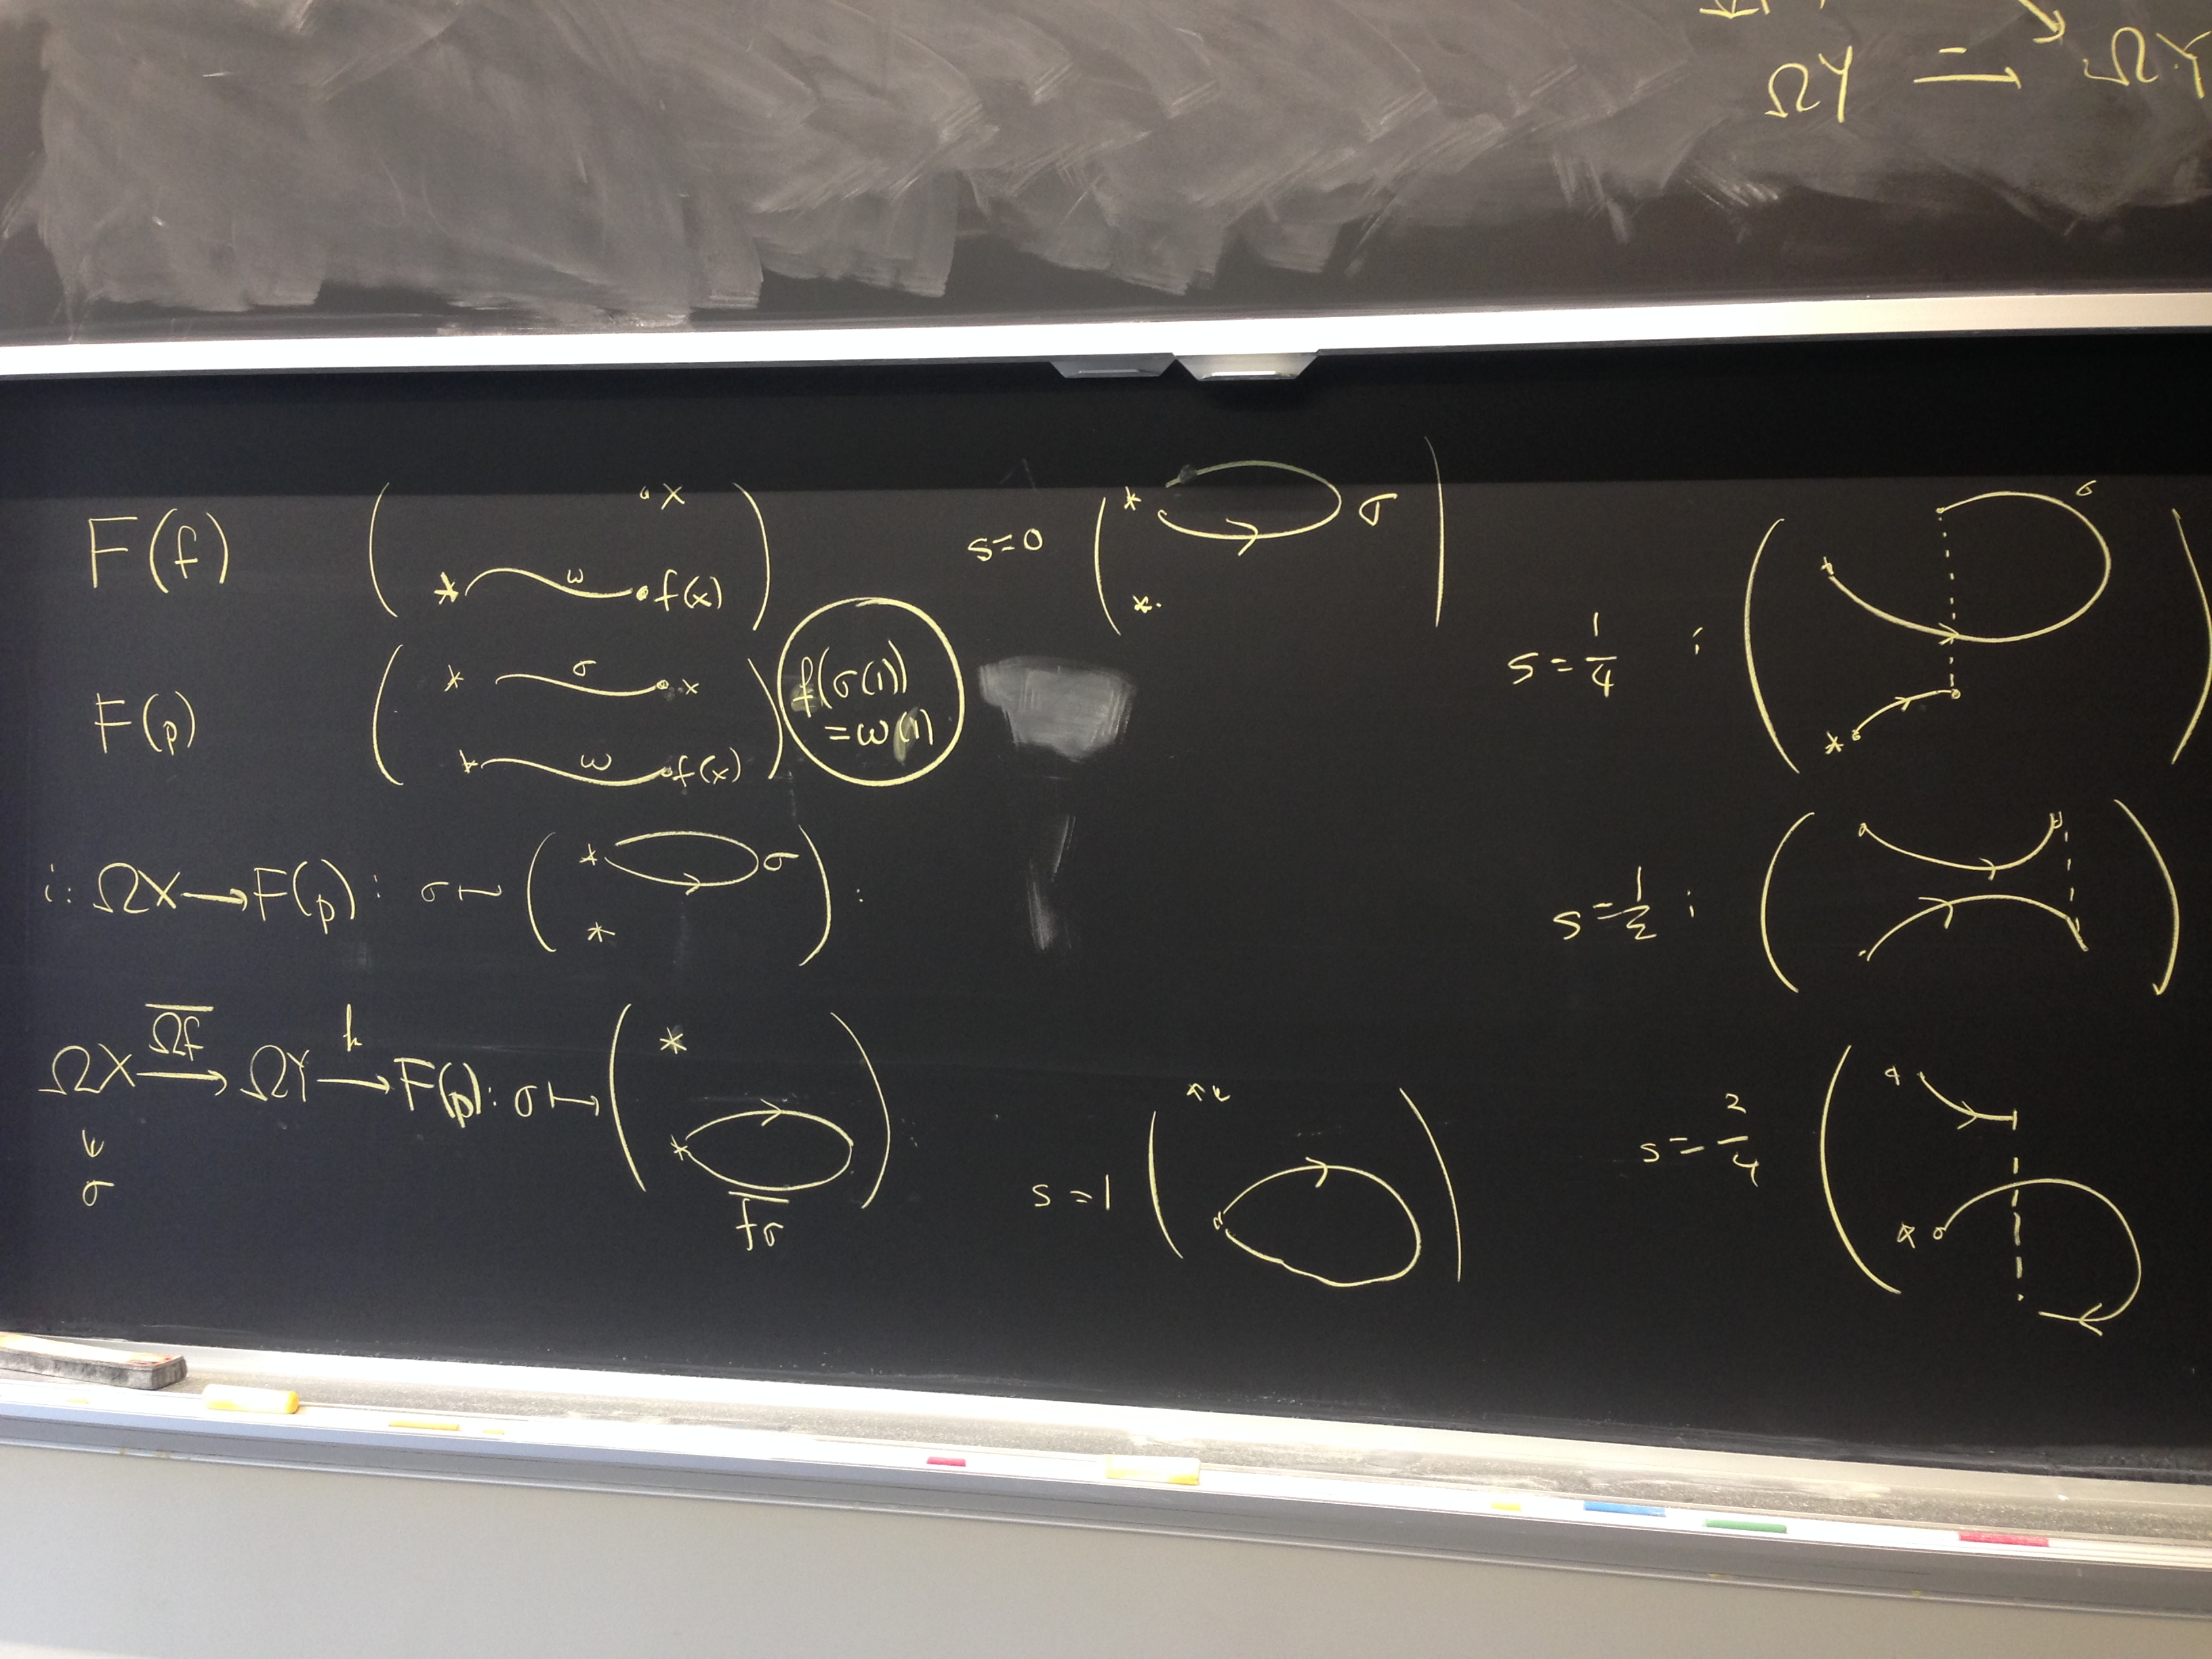
\includegraphics[width=\textwidth]{assets/barratt-puppe}
\caption{A proof of this lemma.}
\end{figure}
\end{proof}
\begin{lemma}
    The following diagram commutes:
    \begin{equation*}
	\xymatrix{
	    & F(\overline{\Omega p_0})\ar@{=}[dd]\ar[dr] & \\
	    \Omega^2 Y\ar[ur]^{i(\Omega p_0)}\ar[dr]_{\overline{\Omega i(p_0)}} & & \Omega X\\
	    & \Omega Fp_0\ar[ur]_{\overline{\Omega p_1}} & 
	    }
    \end{equation*}
\end{lemma}
What is the map $F\overline{\Omega p_0}\to \Omega X$?? We spent some time figuring this out. But you can now apply $[W,-]_\ast$ to the following diagram to get a long exact sequence:
\begin{equation*}
    \xymatrix{
	\cdots\ar[r] & Fp_4\ar[r] & Fp_3 \ar[r] & Fp_2\ar[r] & Fp_1\ar[r]^{p_2} & Ff\ar[r]^{p_1} & X\ar[r]^{f} & Y\\
    \cdots\ar[r] & \Omega Fp_1\ar[r]|{\overline{\Omega p_2}}\ar[u]_{\simeq} & \Omega Fp_0\ar[u]_{\simeq}\ar[ur]|{i(p_2)}\ar[r]|{\overline{\Omega p}} & \Omega X\ar[r]|{\overline{\Omega f}}\ar[u]_{\simeq}\ar[ur]|{i(p_1)} & \Omega Y\ar[u]_\simeq \ar[ur]|{i(p_0)} & &\\
	\Omega^2 X\ar[u]_{\simeq}\ar[r]_{\Omega f} & \Omega Y\ar[u]_{\simeq}\ar[ur]_{\overline{\Omega i(p_0)}} & & &
    }
\end{equation*}

For example, $S^0=\{\pm 1\}$. We get terms like $\pi_0(\Omega^n X)$, because $[S^0,X] = \pi_0 X$. What is $\pi_0(\Omega^n X)$? This is $[S^0,\Omega^n X]_\ast$. Is it clear to you that this is $[S^n,X]_\ast$?

Ok, well, $\Omega^2 X = (\Omega X)^{S^1}$. Because $(S^1)^{\wedge n} = S^n$. So we find that $(\Omega X)^{S^1} = (X^{S^1}_\ast)^{S^1}_\ast = X_\ast^{S^1\wedge S^1} = X_\ast^{S^2}$.

Well, $\Omega X$ is a homotopy group by concatenation. It's a group, but where the axioms hold up to homotopy. It's a group in the homotopy category. Therefore, $\pi_0 \Omega X$ is a group! It's exactly $\pi_1 X$, which you know to be a group. And then, there's this other thing that happens.

You can think of $\pi_n(X) = [S^n,X]_\ast$ as $[(D^n,S^{n-1}),(X,\ast)] = [(I^n,\partial I^n),(X,\ast)]$. If I take $n=2$, for example, how do I take the product of $\alpha,\beta\in \pi_2(X)$? You just literally put them together (when you think of $\pi_2(X) = [(I^2,\partial I^2),(X,\ast)]$. You can play this game; up to homotopy, you can shrink $\alpha$ and $\beta$ to make them as small I want, and then reverse their position and expand them again\footnote{This probably makes no sense without a picture}\todo{Add a picture}. Thus $\pi_2(X)$ is an abelian group.

Thus, when you apply $\pi_0$ to our sequence $\cdots\to\Omega^2 X\to\Omega^2 Y\to \Omega Fp_0\to \Omega X\to \Omega Y\to Fp_0\to \Omega X\to \Omega Y$, you get an exact sequence (of groups when the homotopy groups are $>0$, and of pointed sets when you have $\pi_0$):
$$\cdots\to \pi_2 X\to \pi_2 Y\to \pi_1 Ff\to \pi_1 X\to\pi_1 Y\to\pi_0 Ff\to\pi_0 X\to \pi_0 X$$
